% !TeX root = main.tex

\section{方法}

\subsection{问题定义}

给定包含 $n$ 个连续词的语言片段 $w_1,\ldots,w_n$，
词级神经编码器将第 $i$ 个词对应的 EEG/\allowbreak{}MEG 窗编码为神经表示 $\mathbf z_i$。
上下文模型联合建模若干相邻的 $\mathbf z$，
取目标位置的输出与冻结的文本表示对齐，得到目标词的候选排序；
文本序列解码再结合语言评分，将各词位的候选组织为连续文本。

实验按词窗的时间顺序重放离线数据，仅使用当前已经获得的神经输入。
词级对齐、片段边界和词数视为已知。


\subsection{局部神经上下文}

对目标位置 $i$，取其左侧 $l$ 个和右侧 $r$ 个相邻词，构成局部上下文
\[
\mathbf{Z}_i^{(l,r)}
=(\mathbf{z}_{i-l},\ldots,\mathbf{z}_i,\ldots,\mathbf{z}_{i+r}),
\]
索引在片段边界处截断至 $[1,n]$。
该序列输入上下文 Transformer 模型 $f_{\mathrm{ctx}}$，只取目标位置 $i$ 对应的输出隐状态并经 $L_2$ 归一化，得到上下文神经表示：
\[
\hat{\mathbf{y}}_i^{(r)} = \frac{f_{\mathrm{ctx}}(\mathbf{Z}_i^{(l,r)})_i}{\|f_{\mathrm{ctx}}(\mathbf{Z}_i^{(l,r)})_i\|_2} .
\]
令 $l=r=k$ 即得到半径为 $k$ 的对称窗口，改变 $k$ 可以考察检索性能对上下文范围的依赖。
右侧范围 $r$ 同时决定了目标词需要等待多少后续输入。


\subsection{滚动修正}

每个词的神经窗取其语音起点后 $1\,\mathrm{s}$ 的信号；
下文称某个词窗“到达”，指该窗已完整可用。
目标词 $i$ 的词窗到达时，模型以 $\mathbf Z_i^{(k,0)}$ 给出首次预测；
此后每到达一个后续词窗，就以扩展后的 $\mathbf Z_i^{(k,r)}$ 重新预测，直至 $r=R$：
\[
\hat{w}_i^{(0)}\rightarrow\hat{w}_i^{(1)}\rightarrow\cdots\rightarrow\hat{w}_i^{(R)}.
\]
本文取 $k=R=2$，并将三个可见状态记为
\[
\mathrm{K0}:[-2,0],\qquad\mathrm{K1}:[-2,1],\qquad\mathrm{K2}:[-2,2].
\]
第 $t$ 个词窗到达时，模型给出词 $t$ 的 K0 预测，
同时将词 $t-1$ 和 $t-2$ 分别更新到 K1 和 K2；
可修正区域随 $t$ 向前滚动（图~\ref{fig:rolling_revision_method}）。
片段边界处只使用片段内实际存在的词窗。

\begin{figure}[!htbp]
    \centering
    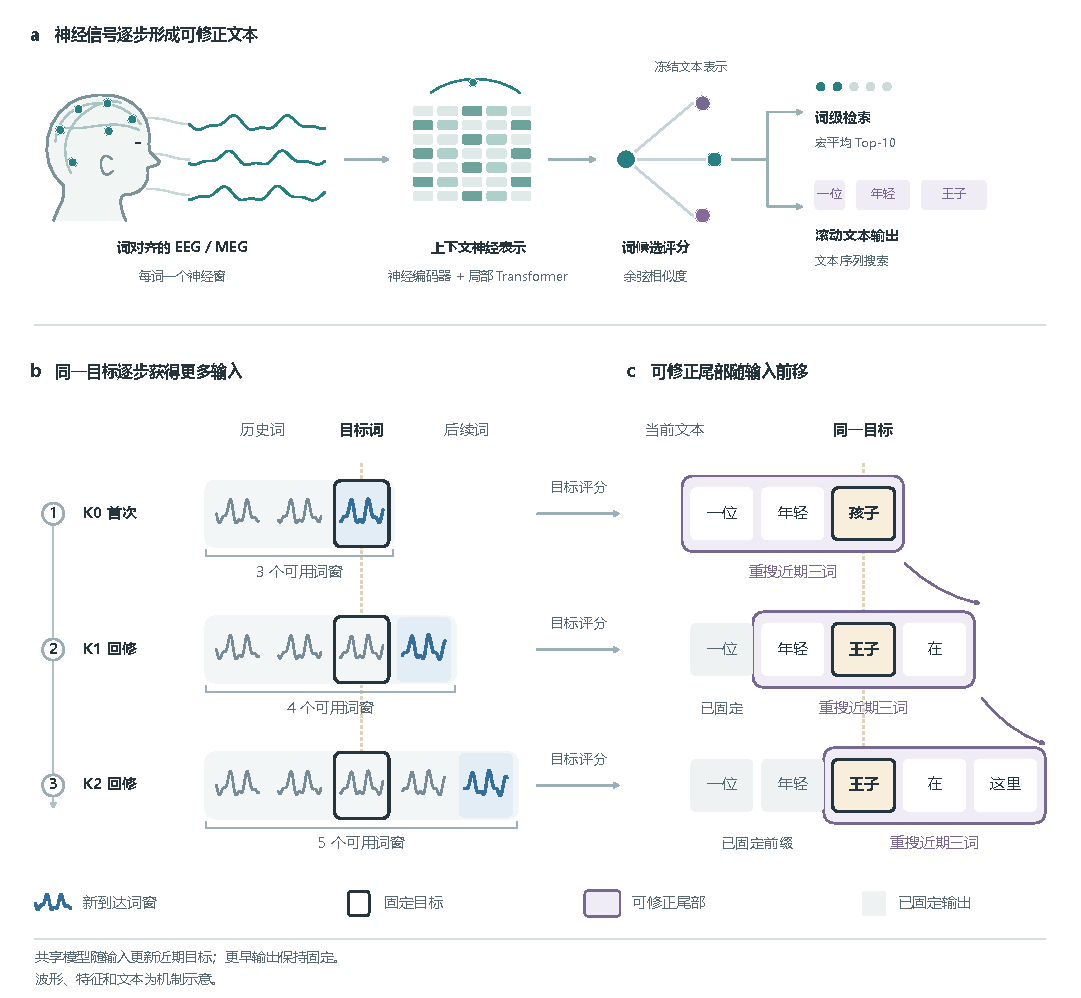
\includegraphics[width=\linewidth]{method_overview_editorial.pdf}
    \caption{滚动修正示意。蓝色为新到达的神经窗，黑框为固定目标，紫色为近期可回修词位，灰色为已固定输出。共享模型随新词窗到达更新近期表示并重新搜索文本。}
    \label{fig:rolling_revision_method}
\end{figure}

\subsection{输入等待}
\label{sec:input_wait}

设词 $i$ 的语音起点为 $\tau_i$，神经窗长度为 $T=1\,\mathrm{s}$。
若目标词最多等待 $R$ 个后续词窗，其最终预测所需输入的可用时刻为
\[
c_i^{(R)}=\tau_{\min(i+R,\,n)}+T .
\]
$R=0$ 对应首次预测，$R\ge n-i$ 对应等待片段末词窗的完整片段解码。
本文报告的总输入等待为 $c_i^{(R)}-\tau_i$。
输入等待按神经输入的可用时间计算，不含模型推断与文本搜索开销。


\subsection{共享滚动训练}
\label{sec:revision_training}

训练分两个阶段。
先训练不含跨词上下文的词模型；
再用其初始化神经编码器，新建上下文模型进行滚动训练。
K0、K1 和 K2 共享同一组参数。

滚动训练按词窗到达顺序模拟预测过程：
第 $t$ 个词窗到达时，同时监督词 $t$ 的 K0、词 $t-1$ 的 K1 和词 $t-2$ 的 K2 预测，
片段边界处不存在的状态跳过。
设批次 $b$ 中含有效目标的状态集合为 $D_b$，
各状态先在其目标上平均对比损失，再等权平均：
\[
\mathcal{L}_b
=\frac{1}{|D_b|}\sum_{r\in D_b}\mathcal{L}_b^{(r)} .
\]
对比负样本取批次内的其他文本目标，并屏蔽与目标相同的词。


\subsection{文本序列解码}
\label{sec:sentence_decoding_method}

参考 \cite{jayalath2025unlocking}，我们将神经候选与语言模型评分结合，
在已知词数的条件下逐词进行束搜索。
每个词位的候选包括两部分：
训练词库 $V$ 中神经相似度最高的若干词，以及语言模型根据当前前缀 $u$ 提出的续写词。
后者可以位于 $V$ 之外，同样由冻结文本编码器获得表示。

在可见状态 $r$ 下，目标位置 $i$ 的归一化神经表示 $\hat{\mathbf y}_i^{(r)}$
与候选词表示 $\mathbf y(w)$ 的余弦相似度经缩放后，
在 $V$ 及当前提出的词库外候选上做 softmax 归一化，得到神经概率 $p_{\mathrm N}$。
候选词的得分为
\[
s_i^{(r)}(w\mid u)
=\log p_{\mathrm N}(w\mid\hat{\mathbf y}_i^{(r)},u)
+\lambda\ell_{\mathrm{LM}}(w\mid u),
\]
其中 $\lambda$ 为语言评分权重，$\ell_{\mathrm{LM}}$ 为加入候选词前后整串文本的对数概率之差。
束搜索逐词累加得分，具体参数见附录~\ref{sec:supp_sentence_settings}。

在此基础上比较表~\ref{tab:strategies} 中的六种策略。
近期重搜保持更早的前缀固定，策略 F 从空前缀开始搜索整个片段。
F-local 与 F 使用相同的完整片段输入等待和整段搜索，
但复用 C 的最终局部表示：内部词位为 K2，末两个词位按片段边界使用 K1 和 K0。
B 用于区分神经表示更新与文本重搜的作用，新词仍以其自身 K0 表示进入搜索。
各策略使用相同的候选构造、语言评分和搜索参数。

\begin{table}[!htbp]
    \centering
    \papertablestyle
    \caption{文本序列解码策略。}
    \label{tab:strategies}
    % Definitions of the six frozen text-decoding strategies; no experimental results.
\begingroup
\papertablestyle
\begin{tabular}{@{}llccc@{}}
\toprule
策略 & 名称 & 神经表示 & 每次重搜词位 & 输出固定时刻 \\
\midrule
A  & 固定输出     & K0                       & 1（当前词） & $c_i^{(0)}$ \\
B  & 固定表示重搜 & K0                       & 3           & $c_i^{(2)}$ \\
C1 & 一次回修     & K0$\to$K1                & 2           & $c_i^{(1)}$ \\
C  & 滚动修正     & K0$\to$K1$\to$K2         & 3           & $c_i^{(2)}$ \\
F  & 完整片段     & 完整上下文               & 整段        & $\tau_n+T$ \\
F-local & 局部整段 & K2                       & 整段        & $\tau_n+T$ \\
\bottomrule
\end{tabular}
\endgroup

\end{table}
